\let\negmedspace\undefined
\let\negthickspace\undefined
\documentclass[journal]{IEEEtran}
\usepackage[a5paper, margin=10mm, onecolumn]{geometry}
%\usepackage{lmodern} % Ensure lmodern is loaded for pdflatex
\usepackage{tfrupee} % Include tfrupee package
\setlength{\headheight}{1cm} % Set the height of the header box
\setlength{\headsep}{0mm}     % Set the distance between the header box and the top of the text
\usepackage{gvv-book}
\usepackage{gvv}
\usepackage{cite}
\usepackage{amsmath,amssymb,amsfonts,amsthm}
\usepackage{algorithmic}
\usepackage{graphicx}
\usepackage{textcomp}
\usepackage{xcolor}
\usepackage{txfonts}
\usepackage{listings}
\usepackage{enumitem}
\usepackage{mathtools}
\usepackage{gensymb}
\usepackage{comment}
\usepackage[breaklinks=true]{hyperref}
\usepackage{tkz-euclide} 
\usepackage{listings}
% \usepackage{gvv}                                        
\def\inputGnumericTable{}                                 
\usepackage[latin1]{inputenc}                                
\usepackage{color}                                            
\usepackage{array}                                            
\usepackage{longtable}                                       
\usepackage{calc}                                             
\usepackage{multirow}                                         
\usepackage{hhline}                                           
\usepackage{ifthen}                                           
\usepackage{lscape}
\begin{document}

\bibliographystyle{IEEEtran}
\vspace{3cm}
\parindent 0px

\title{9.2.3}
\author{EE24BTECH11050 - Pothuri Rahul}
% \maketitle
% \newpage
% \bigskip
{\let\newpage\relax\maketitle}

\renewcommand{\thefigure}{\theenumi}
\renewcommand{\thetable}{\theenumi}
\setlength{\intextsep}{10pt} % Space between text and floats


\numberwithin{equation}{enumi}
\numberwithin{figure}{enumi}
\renewcommand{\thetable}{\theenumi}

\textbf{Question:} \\
What is the solution for the differential equation $y'+\sin{x}=0$
\solution \\
\textbf{Theoretical solution :} \\
by rearranging the given differential equation \\
\begin{align}
\frac{dy}{dx} = - \sin{x} \label{1}
\end{align}
On integrating both sides w.r.to x,
\begin{align}
\int \frac{dy}{dx} dx = \int \brak{- \sin{x}} dx \\
y = \cos{x}+C
\end{align}
\textbf{Solution using Trapezoidal rule :} \\
Consider the equation \eqref{1},
\begin{align}
\frac{dy}{dx} = - \sin{x} \\
dy = -\sin{x}dx
\end{align}
To apply the Trapezoidal rule, we need to convert it into definite integration. For that let us take two points on x-axis $x_n$ and $x_{n+1}$,which are at a small separation h and $y_n , y_{n+1}$ be the values of respectively. \\
\begin{align}
\int\limits_{y_n} ^{y_{n+1}} dy = \int\limits_{x_n} ^{x_{n+1}} \sin{x} dx
\end{align}
By Trapezoidal rule,We can approximate it as,
\begin{align}
y_{n+1}-y_n = \frac{1}{2} \times h \brak{ \sin{x_n}+\sin{x_{n+1}}}
\end{align}
Where,
\begin{align}
h = x_{n+1} - x_n
\end{align}
By taking initial conditions as $x_0 = 0,y_0 = 1$ and plotting the points resulted in this algorithm will give the approximate graph for the given differential equation \eqref{1} 

\begin{figure}[htbp] % Positioning options: here, top, bottom, page
    \centering
    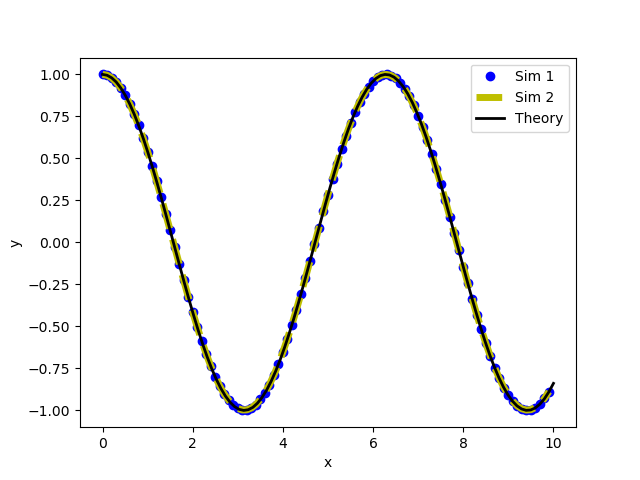
\includegraphics[width=\textwidth]{figs/plot.png} % Replace "filename" with your image file
    \caption{Plot}
\end{figure}






\end{document}
